\documentclass{article}

\usepackage{amsmath,graphicx,parskip,mathrsfs,subfigure}
\usepackage{fancyhdr}
\usepackage{amsthm,amssymb}
\usepackage{setspace}
\usepackage{epstopdf}
\usepackage[left=3cm,right=3cm,top=3cm,bottom=3cm]{geometry}

\pagestyle{fancy}
\lhead{Samuel Huberman}
\chead{MSE1022:HW1}
\rhead{999157923}

\begin{document}
\section{Part A}

1. The Young's modulus is given by the the linear regression of the elastic portion of the stress-strain data, giving $E=9534.97$ MPa. The yield stress is defined as the stress at which the stress-strain curve deviates from the initial linear behaviour, giving $\sigma_{yield}=930.61981$ MPa. The ultimate stress is defined as the maximum stress achieved: $\sigma_{ultimate}=1119.7594$ MPa. These values are far from the experimentally observed values of bulk gold $E=79$GPa and $\sigma_{yield}=120$ MPa. \\
\begin{figure}[h!]
\centering
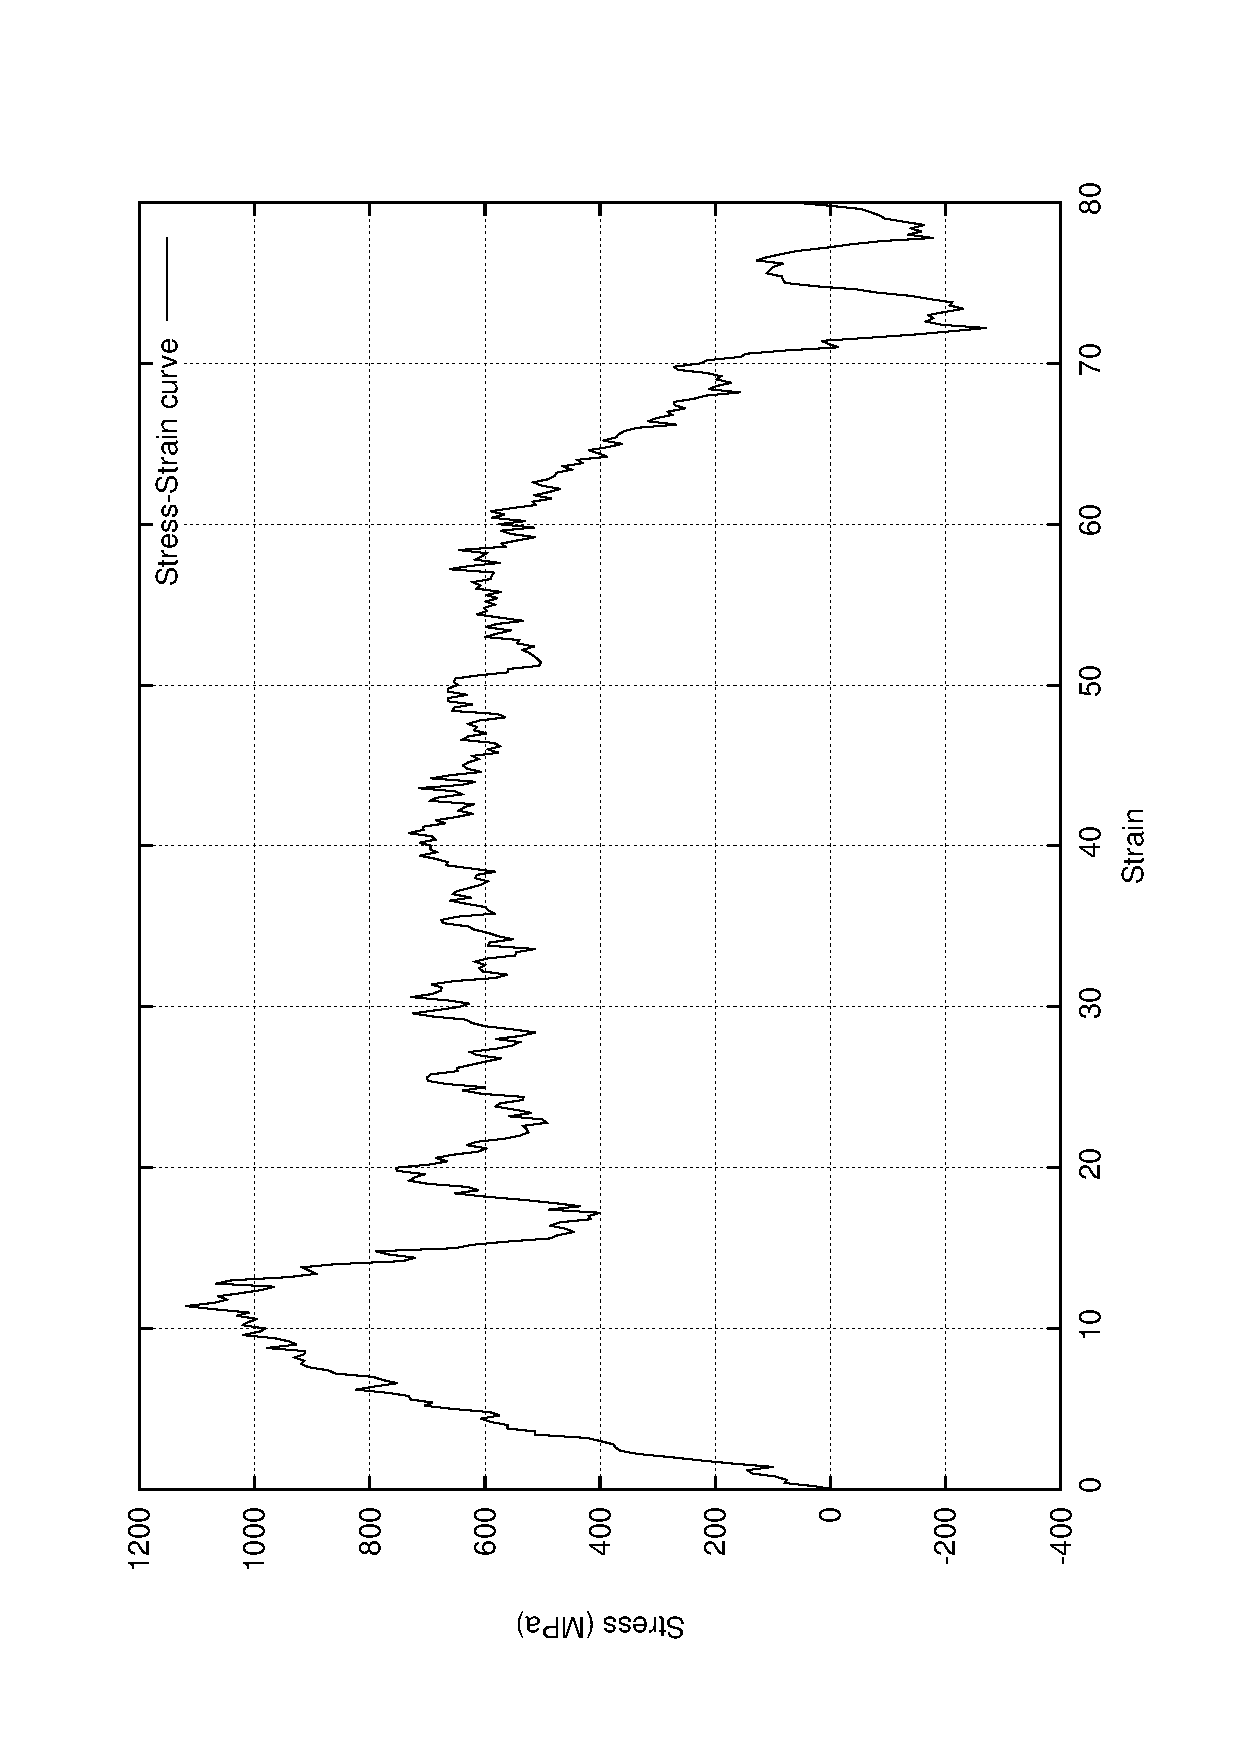
\includegraphics[totalheight=0.5\textheight, angle=-90]{se_curve1}
\caption{Stress-strain plot for $\dot{\epsilon}=10^9$ $[sec^-1]$}
\label{fig:aNicePicture}
\end{figure}
\\
2.
\begin{center}
\begin{tabular}{|c|c|c|}
  \hline
  Strain Rate [$sec^-1$] & Young's modulus [MPa] & Yield Stress [MPa] \\
  \hline
  1E9 & 11597.8   & 939.33836   \\ \hline
  5E8 & 12672.2   & 952.36519 \\ \hline
  1E8 & 13901    &  814.3793   \\ \hline
\end{tabular}
\end{center}\
\begin{figure}[h!]
\centering
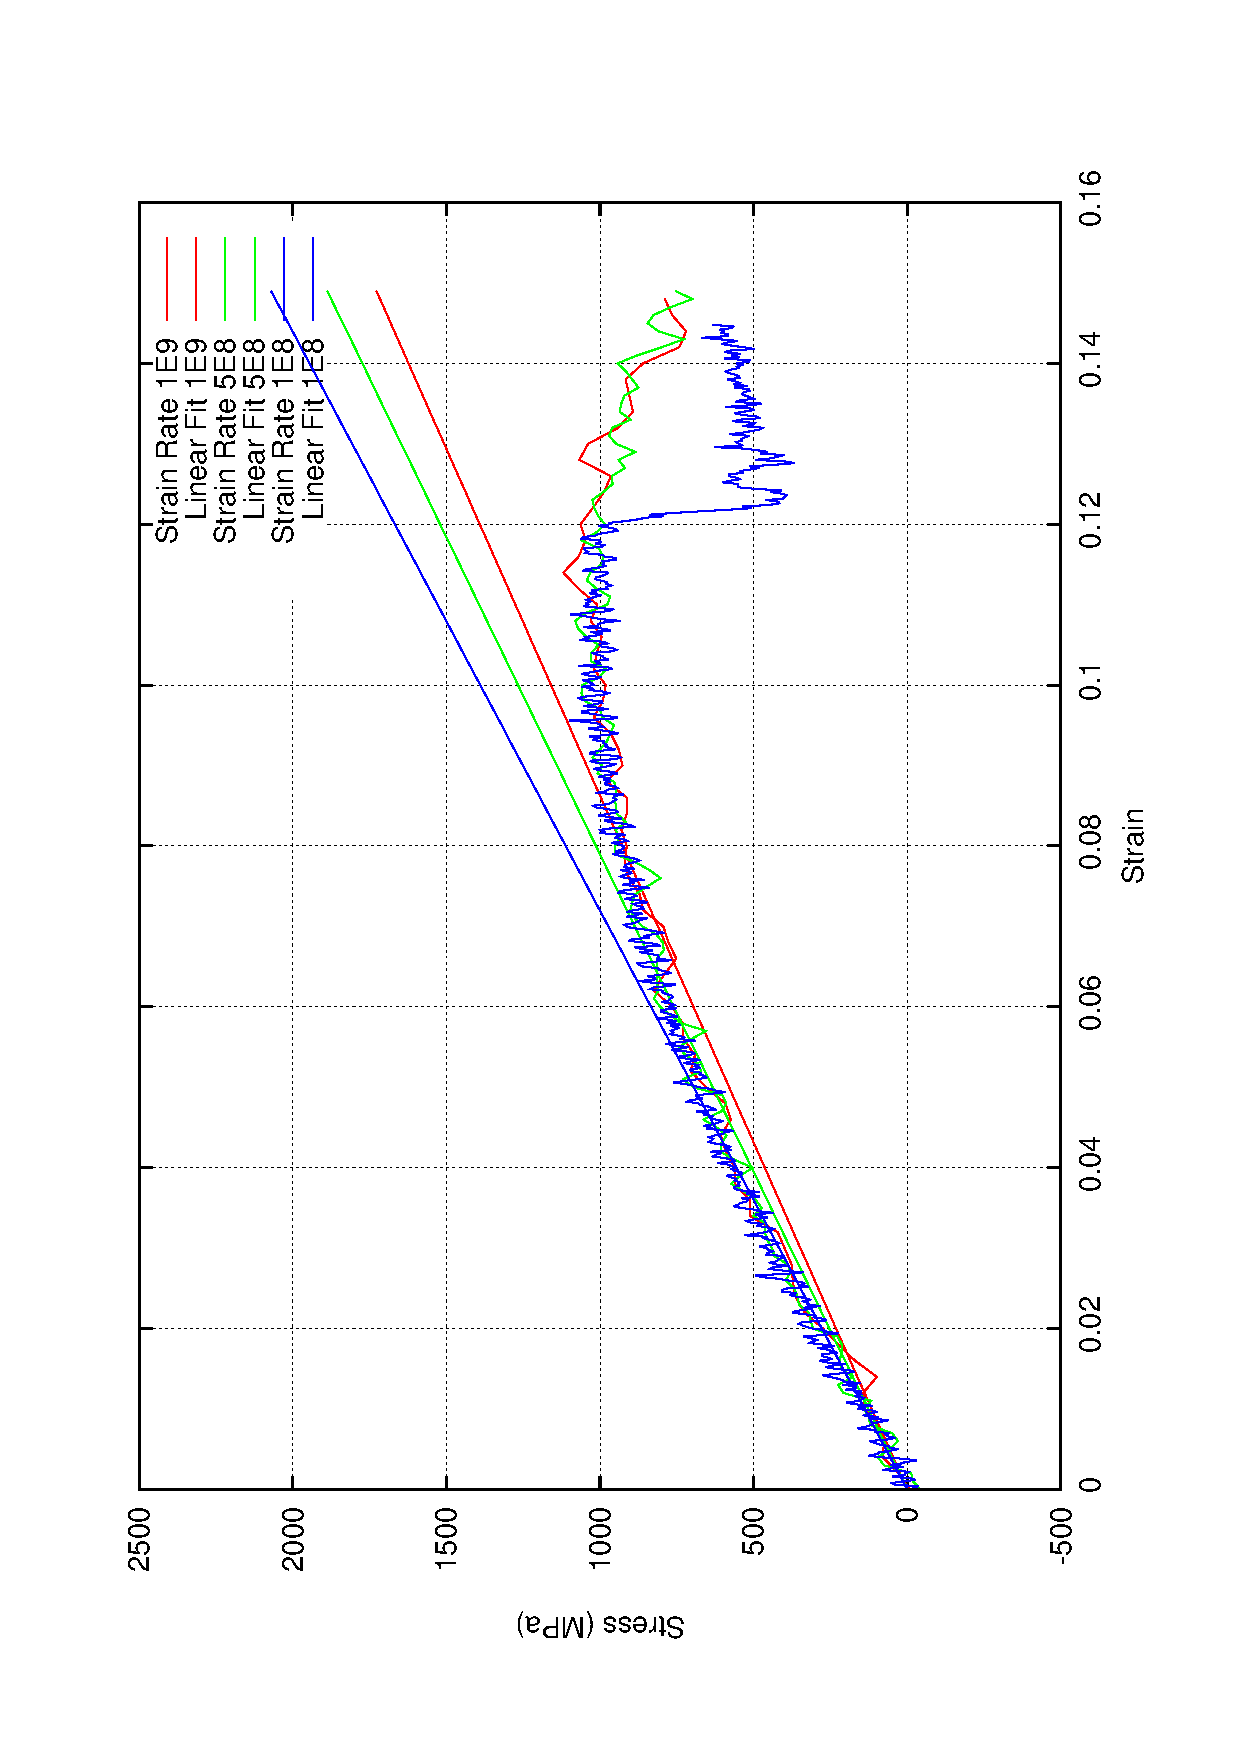
\includegraphics[totalheight=0.5\textheight, angle=-90]{se_curve2}
\caption{Stress-strain plot for 3 $\dot{\epsilon}$ }
\label{fig:aNicePicture}
\end{figure}
In a bulk material, we would not expect the Young's modulus to depend upon the strain rate, as it is a material property and independent of (realistic) strain rates. However, the exception is the rule when it comes to nano-scale systems. Thus, there may exist some deviation from the general rule of linear dependence of tensile stress upon applied strain as a consequence of the size of sample.
\\
3.\begin{center}
\begin{tabular}{|c|c|c|}
  \hline
  Temperature & Young's modulus [MPa] &Yield Stress [MPa]\\
  \hline
  100 & 13436.2    & 1043.7649  \\ \hline
  200 & 12607  & 964.99698  \\ \hline
  300 & 11597.8 & 861.17303  \\ \hline
\end{tabular}
\end{center}
\begin{figure}[h!]
\centering
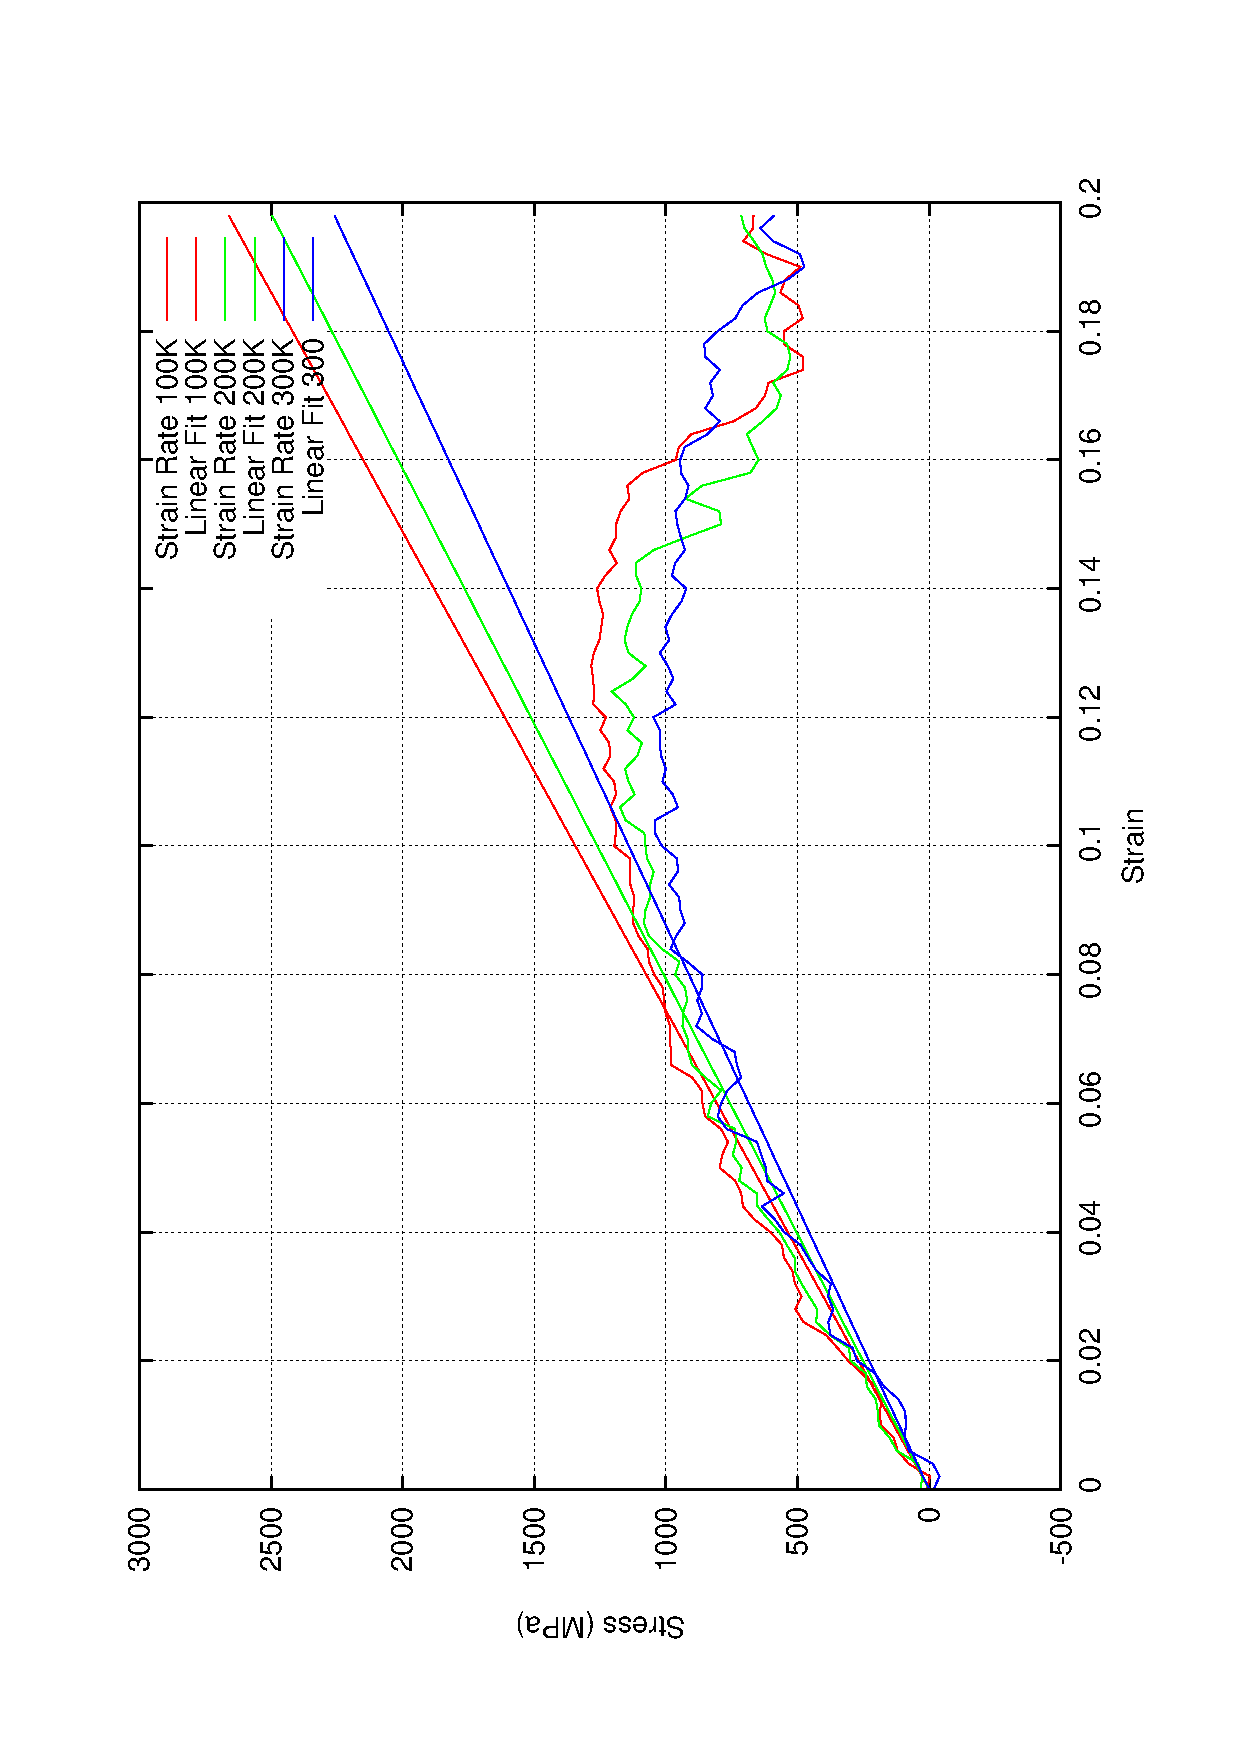
\includegraphics[totalheight=0.5\textheight, angle=-90]{se_curve3}
\caption{Stress-strain plot at 3 temperatures }
\label{fig:aNicePicture}
\end{figure}
As temperature increases, the average distance between atoms increases because of the anharmonicity of the interatomic potential (i.e.: thermal expansion). This increase in interatomic spacing corresponds to a decrease of the potential energy of each atom and an increase in kinetic energy. Therefore, as temperature increases, the force experienced on one atom due to the presence of its neighbours weakens. The manifestation of this is observed macroscopically in the decrease in Young's modulus and Yield stress with increasing temperature.\\
4.
\begin{figure}[h!]
\centering
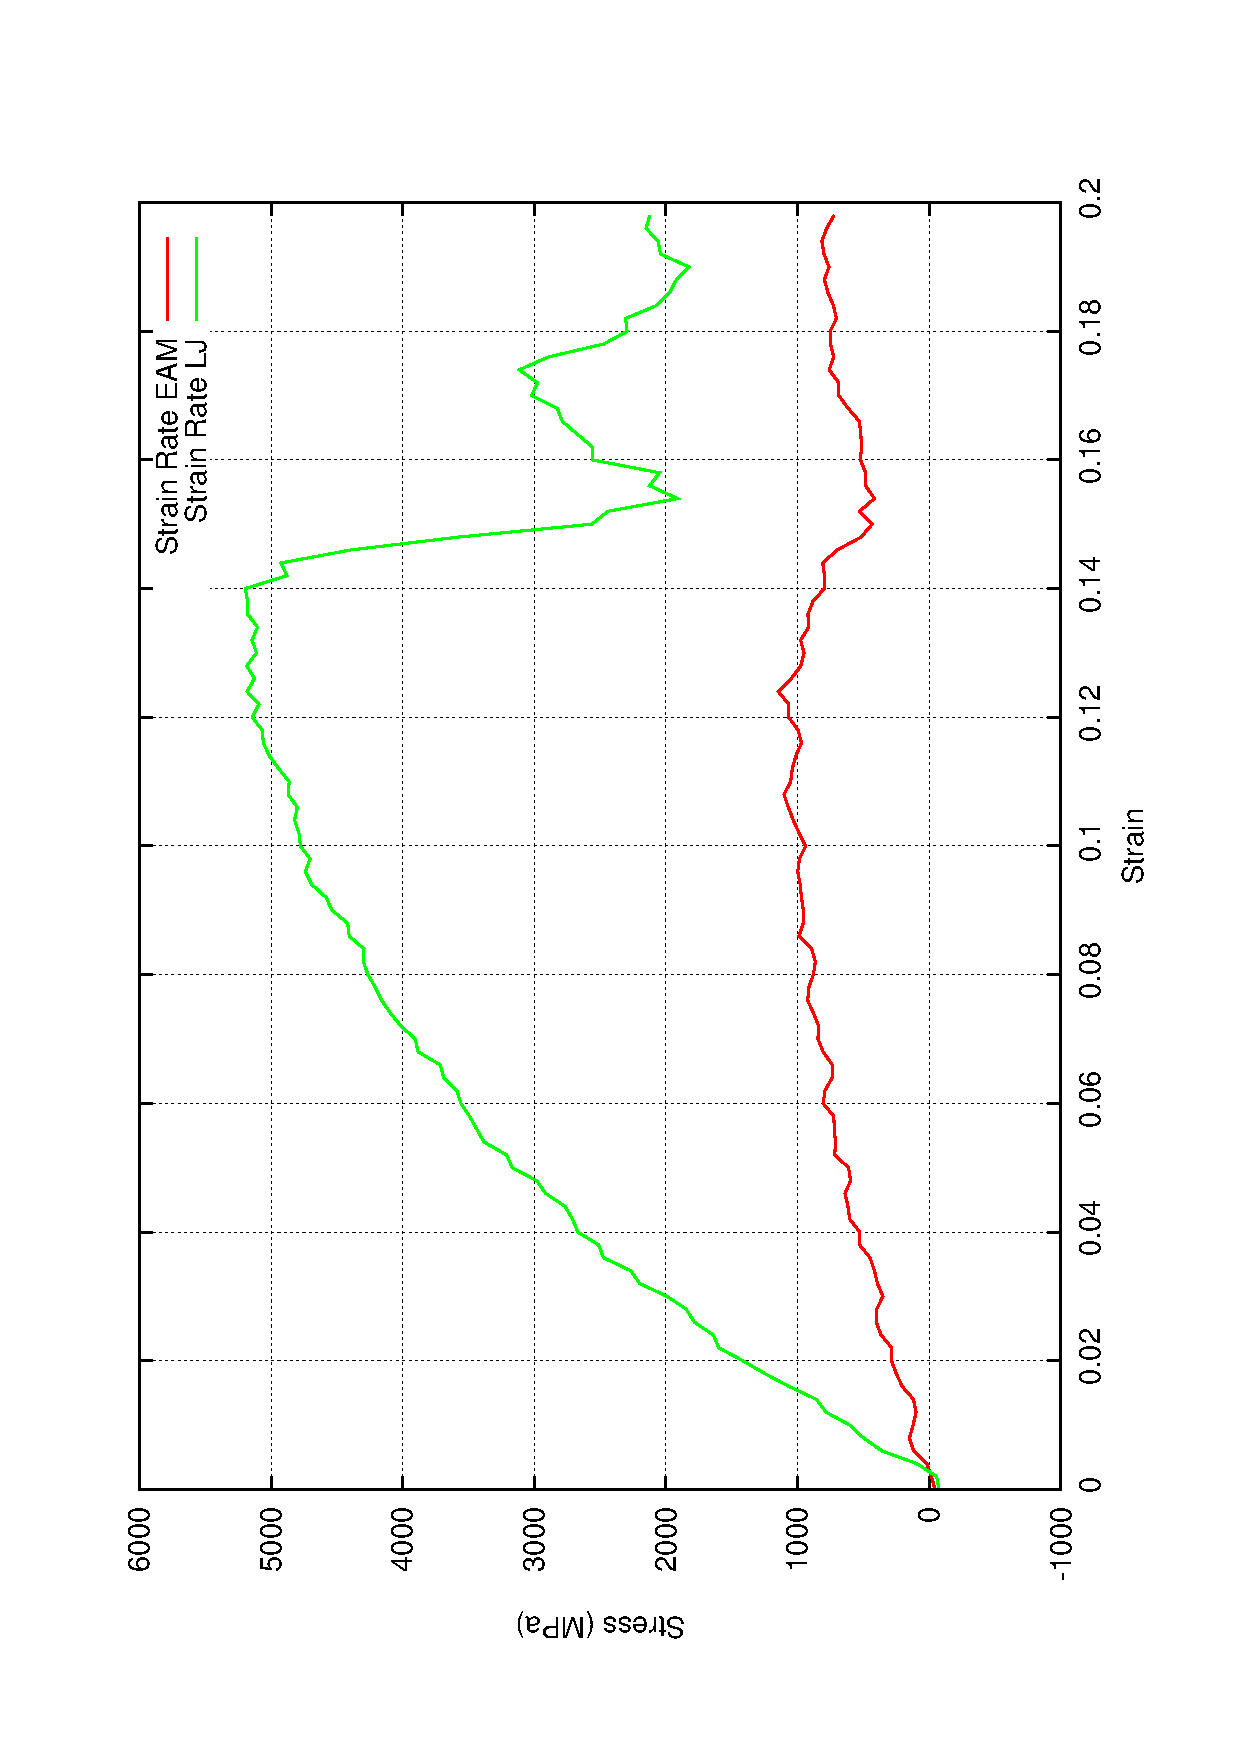
\includegraphics[totalheight=0.5\textheight, angle=-90]{se_curve4}
\caption{Stress-strain plot using LJ, EAM }
\label{fig:aNicePicture}
\end{figure}

\begin{figure}[h!]
\centering
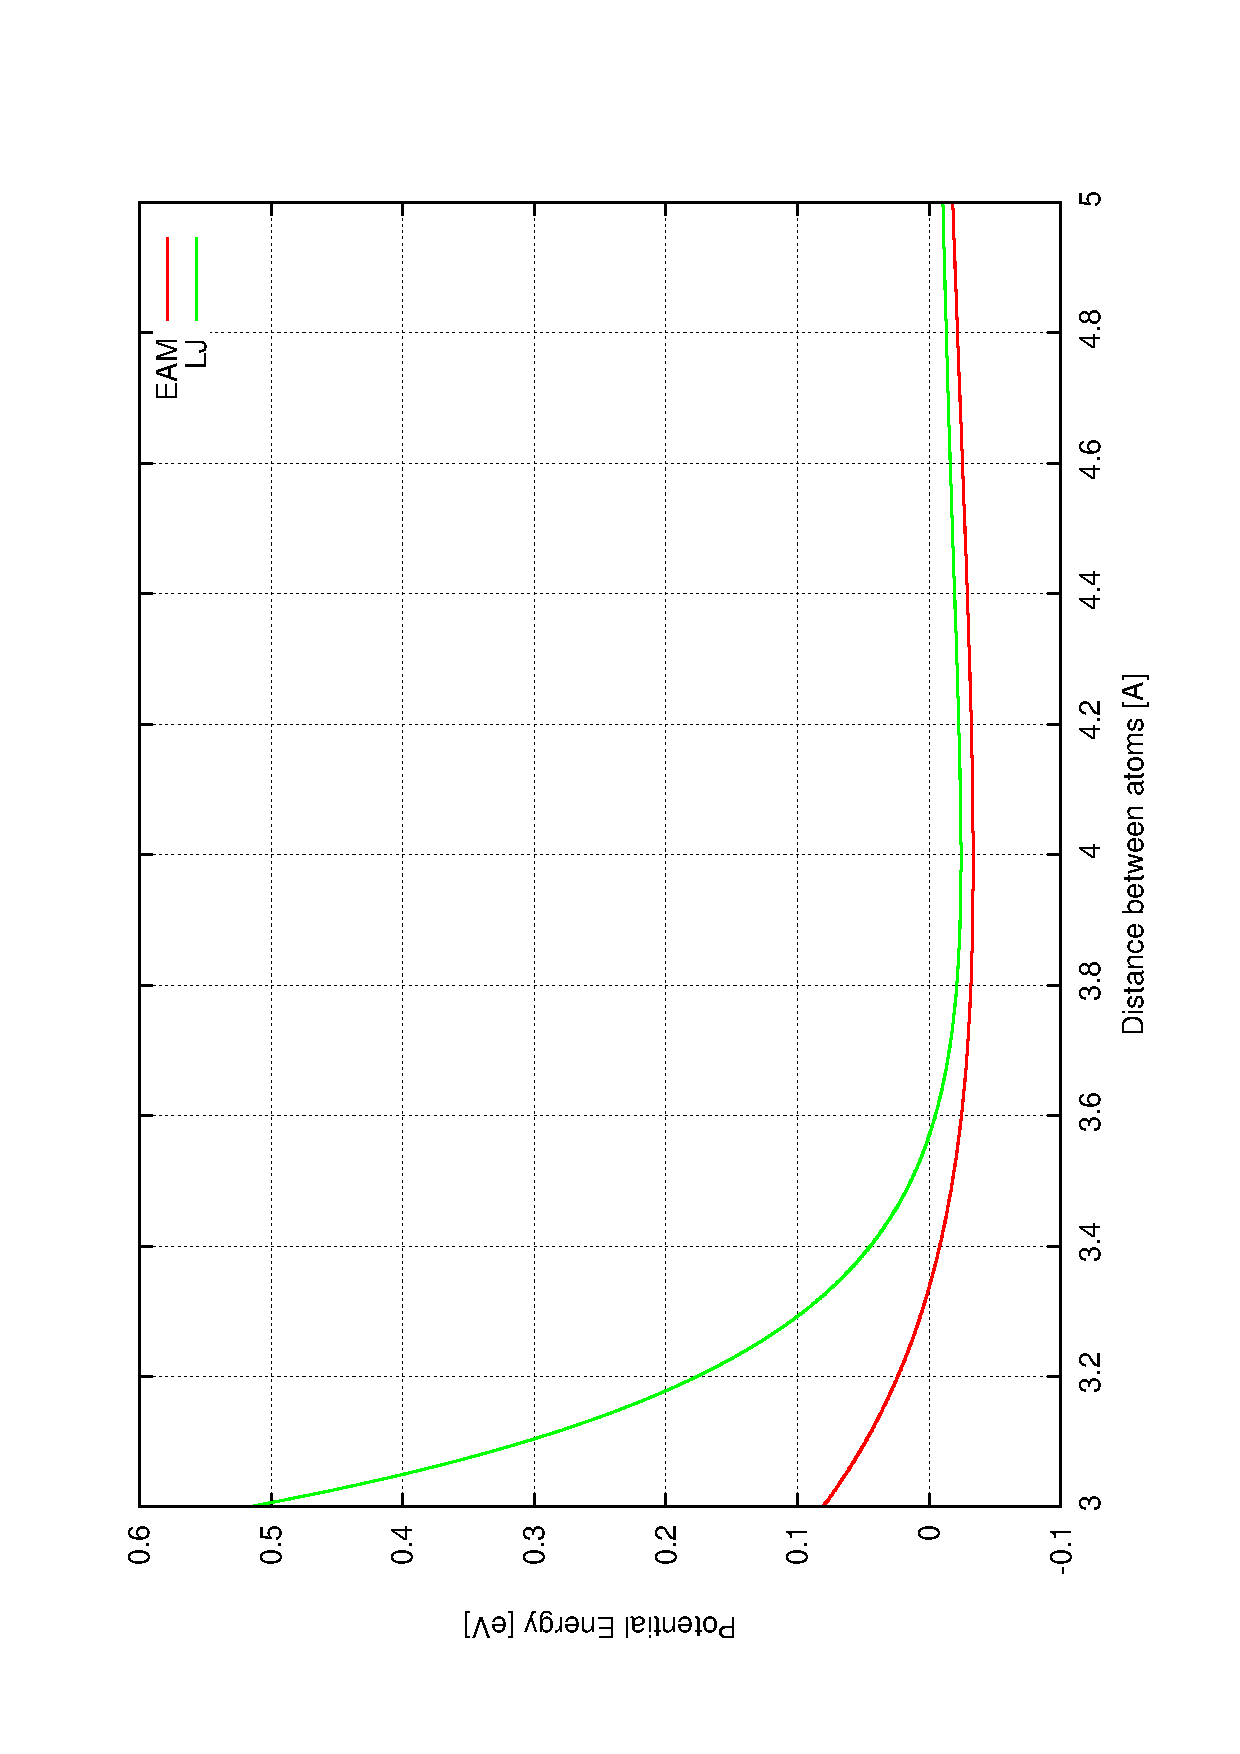
\includegraphics[totalheight=0.5\textheight, angle=-90]{disp_curve}
\caption{LJ v EAM}
\label{fig:aNicePicture}
\end{figure}
At first glance Figure 4 and Figure 5 appear to be at odds with each other. How can a weaker potential (LJ) result in a greater Young's modulus and yield stress while a stronger potential (EAM) has a smaller Young's modulus and yield stress? The plots do not tell the entire story. In MD, the user is required to define the range beyond which the potential does not act. For the LJ potential, the cutoff distance is typically chosen to be $2.5\sigma$, while the EAM potential varies depending upon the implementation. In this scenario, the LJ implementation had a greater cutoff distance than the EAM. Thus LJ atoms continued to experience neighbouring potentials when far apart, while EAM atoms would breakoff once the cutoff distance was surpassed, leading to an overall weaker material. From this it is clear, that the selection of the proper potential is of the utmost importance in order to provide meaningful results.

\section{Part B}

1.
\begin{figure}[h!]
\centering
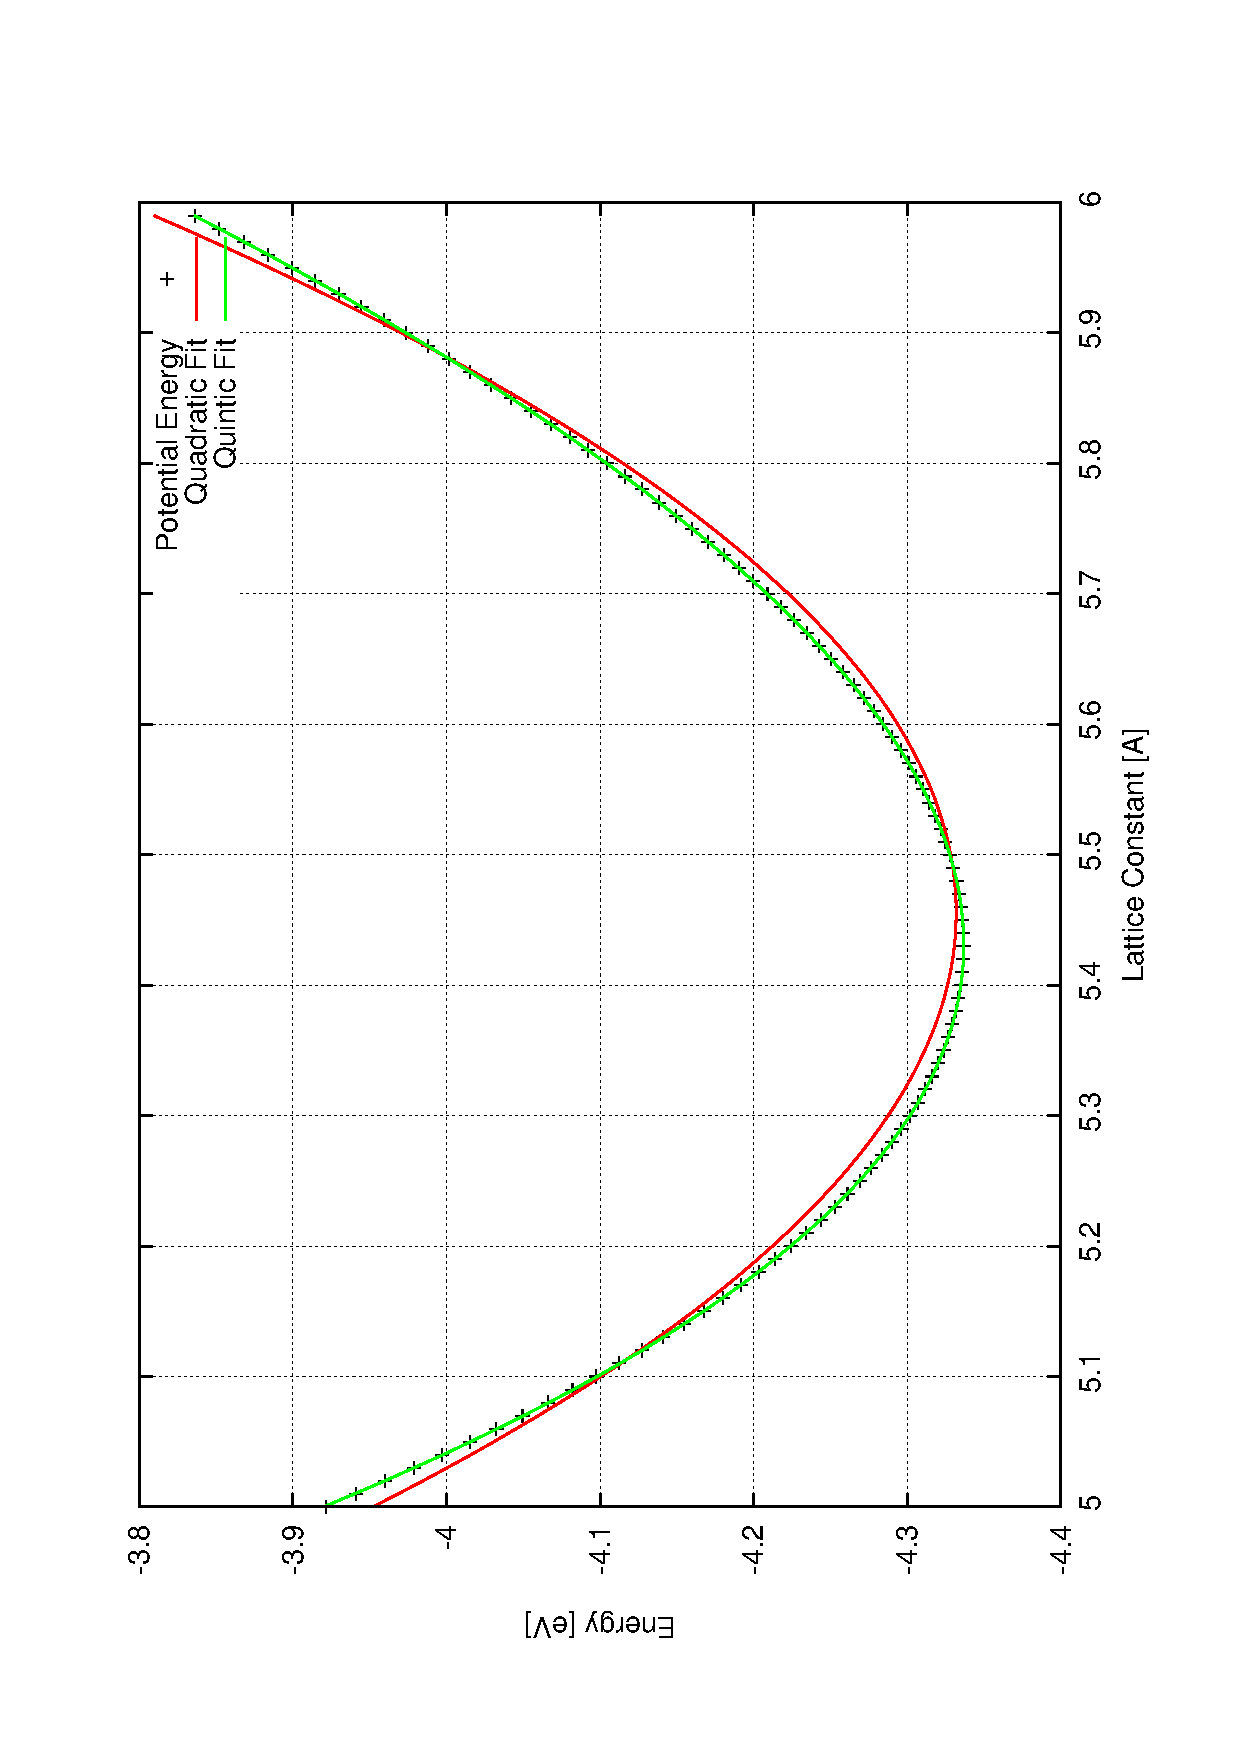
\includegraphics[totalheight=0.5\textheight, angle=-90]{pe_curve}
\caption{Equilibrium lattic constant of silicon}
\label{fig:aNicePicture}
\end{figure}
From the plot, we find that the equilibrium lattice constant is $a_0=5.43085$ A.\\

2.
\begin{center}
\begin{tabular}{|c|c|c|}
  \hline
  Fit & Parameters & Bulk Modulus [$eV/A^3$]\\
  \hline
  Quadratic & $50.1183-19.961*a+1.82939*a^2$ & 16.17\\ \hline
 Quintic &  $-700.047+719.002*a-284.026*a^2+54.422*a^3-5.10833*a^4+0.189352*a^5$ & 22.67 \\ \hline
\end{tabular}
\end{center}\\
These results do not coincide with the observed bulk modulus of 0.63 $eV/A^3$ for silicon.\\
3.
\begin{center}
\begin{tabular}{|c|c|}
  \hline
  Atoms & Total Potential Energy [eV]\\
  \hline
  216  & -936.70558\\ \hline
  215  & -928.03238 \\ \hline
\end{tabular}
\end{center}\\
With the above results, we find $E_{coh}=-4.3365$ eV and $E_{vac}= 2.9172$ eV. This result is in good agreement with Fukata et al. who experimentally determined $E_{vac}= 4.0$ eV using a quenching method [1]. This difference can be attributed to the use of the Stillinger-Weber potential, which will not sufficiently account for the effect of the missing electrons. A more rigourous approach would be to use DFT to determine $E_{vac}$. \\
4.
\begin{center}
\begin{tabular}{|c|c|}
  \hline
  Atoms & Total Potential Energy [eV]\\
  \hline
216  & -936.70558 \\ \hline
217  & -935.65601 \\ \hline
\end{tabular}
\end{center}\\
With the above results, we find $E_{self-int}= 3.954$ eV. This result is in good agreement with Leung et al. who find, using DFT and QMC, $E_{self-int}= 3.31 $ to $5.78$  eV depending upon the location of the interstitial atom relative to the unit cell and the computational technique [2].\\
\newpage
5.
\begin{center}
\begin{tabular}{|c|c|c|}
  \hline
  Boundary & Atoms & Total Potential Energy [eV]\\ \hline
 p p p  &   216   &   -936.7056    \\ \hline
 p s p  &   234   &   -936.7056     \\ \hline     
\end{tabular}
\end{center}
The surface energy cannot be properly inferred from this approach.\\
\section*{References}
\begin{spacing}{1.0}
\small
\noindent
[1] N. Fukata, A. Kayusa and M. Suezawa, Jpn. J. Appl. Phys. \textbf{40}, 854 (2001).\\
[2] W. K. Leung, R. J. Needs, G. Rajagopal, S. Itoh and S. Ihara, Phys. Rev. Lett. \textbf{83}, 2351 (1999).
\newpage
\section*{LAMMPS input scripts}
\subsection*{Part A}
\begin{verbatim}
# Deformation and stress-strain curve for Au nanowire
# Basic settings
#label loop_lattconst
#variable x loop 10000
#variable y equal 3.00+0.0001*${x}
units metal
atom_style atomic
boundary m m p
# Geometry
lattice fcc 4.08 origin 0 0 0 orient z 1 1 0 orient x 0 0 -1 orient y -1 1 0
region box block 0 10 0 5 0 40 units lattice side in
create_box 1 box
create_atoms 1 box
region 1  prism 5.1 10.0 0 5 -1 1000 10 0 0
region 2  prism -1.0 4.9 0 5 -1 1000 -10 0 0
region 3  prism 14.9 20.0 0 5 -1 1000 -10 0 0
region 4  prism -20 -4.5 0 5 -1 1000 10 0 0
group del1 region 1
group del2 region 2
group del3 region 3
group del4 region 4
##### Trim corners
delete_atoms group del1
delete_atoms group del2
delete_atoms group del3
delete_atoms group del4
# Specify inter-atomic potential
pair_style eam
pair_coeff * * Au_u3.eam
#mass 1 197
#pair_style		lj/cut 6.4225
#pair_coeff		1 1 0.458 2.569
#pair_modify          shift yes

neighbor 1.5 bin
neigh_modify every 1 delay 1
# Thermal equilibrium at 300K
velocity all create 300 20199349 dist gaussian
velocity all zero linear
velocity all zero angular

thermo 200
#thermo_style custom step atoms temp pe lx ly lz pzz press
thermo_style custom step atoms temp pe lz pzz 
thermo_modify lost warn norm yes flush yes
timestep 0.005 #ps
#dump 1 all cfg 20000 initialpos.*.cfg id type xs ys zs # Visualize with AtomEye
fix 1 all npt temp 300.0 300.0 10.0 z 0.0 0.0 10.0 drag 2.0
run 20000
# Tensile loading
unfix 1
#undump 1
reset_timestep 0
compute MyTemp all temp
compute Mype all pe
compute peratom all stress/atom
#compute peatom all pe/atom
#compute	pe all reduce sum c_peatom
compute MyDisp all displace/atom 
# Computing time-averaged quantities - T & pe
fix ThermoAve all ave/time 1 100 200 c_MyTemp c_Mype
fix AveDz all ave/spatial 1 100 200 z center 500.0 c_MyDisp[3] norm all file disp.txt
thermo 200
thermo_style custom step atoms f_ThermoAve[1] f_ThermoAve[2] lz vol pzz pe
#thermo_style custom step atoms lz pzz pe
thermo_modify lost warn norm yes flush yes
fix 1 all nvt temp 300.0 300.0 10.0
#log 	1E9e_300K_LJ.txt
#fix 2 all deform 200 z erate 0.0001 # strain rate = 0.0001/ps = 10^8/sec
fix 2 all deform 200 z erate 0.001 # strain rate = 0.001/ps = 10^9/sec
#dump 2 all cfg 20000 pos.*.cfg id type xs ys zs # Visualize with AtomEye
#dump 2 all cfg 5000 pos.*.cfg id type xs ys zs # Visualize with AtomEye
#dump 2 all xyz 50000 Au_*.xyz id type c_MyDisp# Visualize with MDL
#dump_modify 2 element Au
#run 500000
run 100000
#next x
#jump si.lam
#jump si.lam loop_lattconst
\end{verbatim}
\subsection*{Part B}
\begin{verbatim}
#sieq.lam
#label loop_lattconst
#variable x loop 10000
#variable y equal 5.300+0.0001*${x}
clear
units metal
atom_style atomic
boundary p s p
#boundary p p p

lattice diamond 5.43085

region box block 0 3 0 3 0 3
create_box 1 box
create_atoms 1 box
#delete_atoms porosity box 0.00463 482793
create_atoms 1 single 0.7 0.3 0.3

pair_style sw
pair_coeff * * Si.sw Si
mass 1 28
neighbor 1.0 bin
neigh_modify every 1 delay 5 check yes

velocity all create 1 20199349 dist gaussian
velocity all zero linear
velocity all zero angular

#log 	si_$x.lammps
timestep 0.005
thermo 1000
thermo_style custom step atoms temp pe ke etotal press vol
#dump 1 all cfg 1 Si_$x.cfg id type xs ys zs
fix 1 all nvt temp 1.0 1.0 1.0
run 20000
#run 100
unfix 1
fix 1 all box/relax iso 0.0 vmax 0.001
run 20000
#fix 1 all nvt temp 0.0 0.0 0.0
minimize 0 1.0e-8 1000 1000
min_style sd
#run 1000

#next x
#jump si.lam
#jump si.lam loop_lattconst
\end{verbatim}
\end{document}

